%!TEX root = ../SciVis.tex

 Height plots are typically used to visualize scalar functions defined over (planar) 2D domains by plotting the function values along the third (z) dimension. 
 
 scaled value between 0 and a maxheight value. clamping and scaling. 
 
 
 calculated surface normals 
 
 calculated vertex normals based on averaging surface normals
Figure~\ref{fig:figures_heightplot_normalization}
 Figure~\ref{fig:heighplot_densityNormals}
 \begin{figure}[htbp]
    \centering
        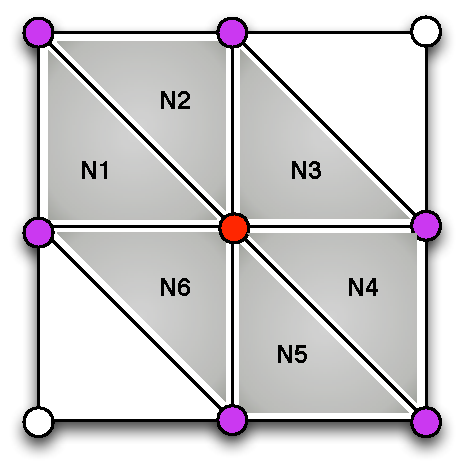
\includegraphics[height=3in]{figures/heightplot/normalization.pdf}
    \caption{In order to calculate the vertex normal (red), the surface normals of the adjacent triangles are averaged.}
    \label{fig:figures_heightplot_normalization}
 \end{figure}
 
 fluid density rho, the velocity magnitude | v |, and the force magnitude | f 
 
 
 
one of the scalar fields named above  -> extra input field to be able to visualize to different scalar sets

viewpoint selection 
tilt the world to get a top- bottom view (rotation around x)
distance of  camera is adjustable
specify three axis of the direction to look at 
euler angles  were considered 


Finally, use the color of the plot to show a separate scalar field, via the already familiar color mapping technique. For example, the plot height can show rho, and the plot color can show | f |
figure 17 shows that it can be confusing to visualize different datasets as the colormap creates an artificial shaded topology that does not correlate with the actual heightmap and thus confuses the viewer. 
\ref{fig:heighplot_densityVelocity}


Figure~\ref{fig:figures_heightplot_densitydensitybanding}


\begin{figure}[htbp]
\centering
\begin{minipage}[t]{0.48\textwidth}
        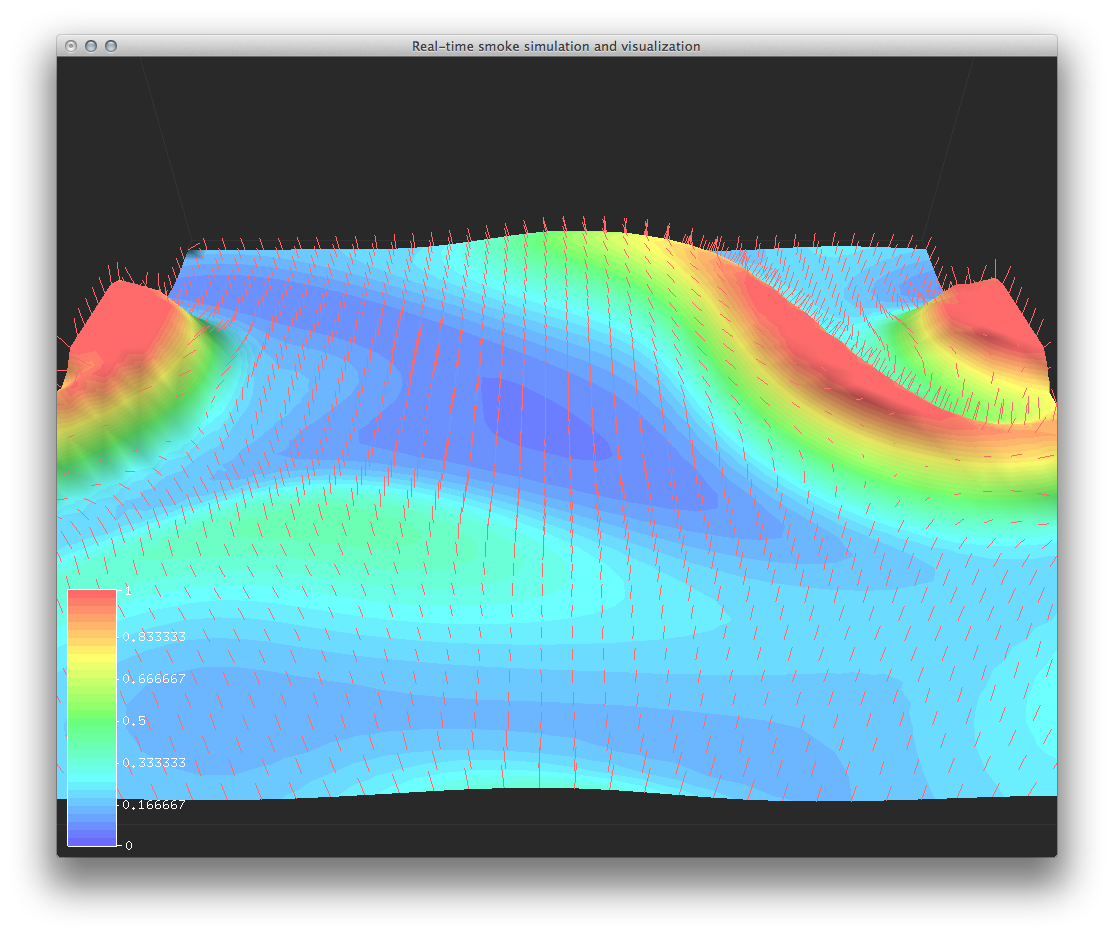
\includegraphics[height=3in]{figures/heightplot/densitynormals.png}
        \caption{The height plot and colormap both shows the density. The calculated vertex normals are shown as little red pikes facing into the direction of the normal.}
\label{fig:heighplot_densityNormals}
\end{minipage}\hspace{.04\textwidth}%
\begin{minipage}[t]{0.48\textwidth}
 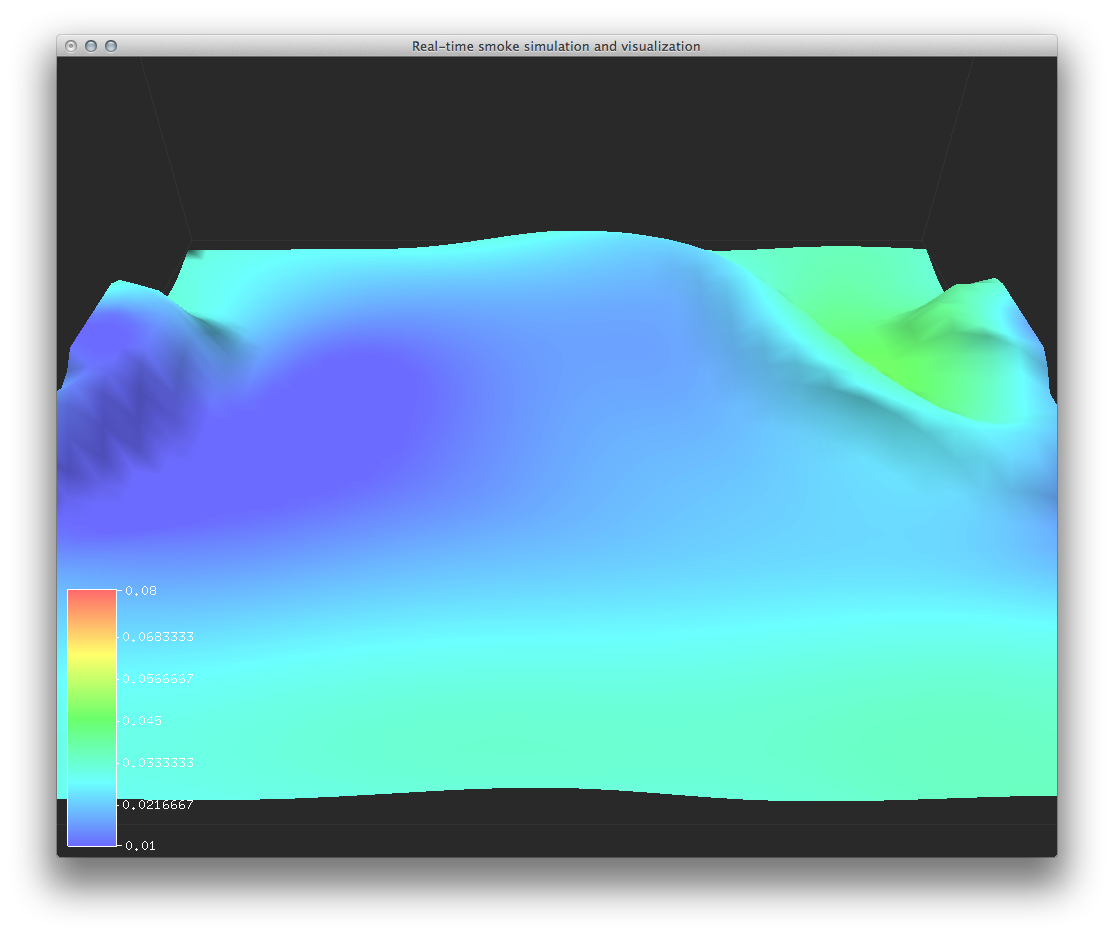
\includegraphics[height=3in]{figures/heightplot/densityvelocity.png}
    \caption{The height plot shows density while the colormap visualizes the velocity. It can be seen that the topological peaks and color peaks are not aligned }
    \label{fig:heighplot_densityVelocity}
\end{minipage}
\end{figure}

\begin{figure}[htbp]
    \centering 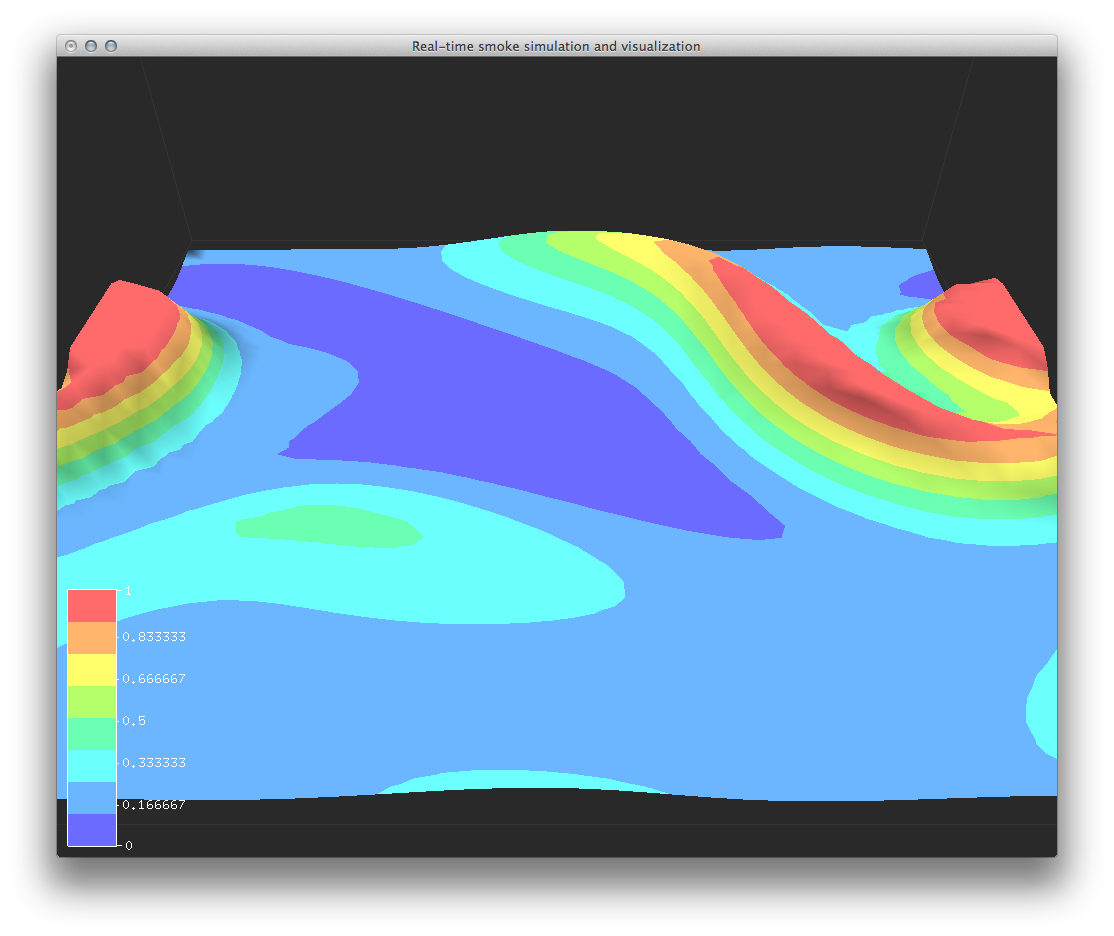
\includegraphics[height=3in]{figures/heightplot/densitydensitybanding.png}
    \caption{Reducing the number of colors makes it easy to compare the height of different peaks but it comes at the cost of a less accurat inverse mapping.}
    \label{fig:figures_heightplot_densitydensitybanding}
\end{figure}



